% !TEX encoding = UTF-8
% !TEX TS-program = pdflatex
% !TEX root = ../tesi.tex
% !TEX spellcheck = it-IT

%**************************************************************
\chapter{Il progetto nella strategia aziendale}
\label{cap:il-progetto-nella-strategia-aziendale}
%**************************************************************
\intro{Questo capitolo fornisce una descrizione dettagliata del progetto di stage, e dei motivi che hanno spinto l'azienda a proporlo oltre che i benefici derivati da tale progetto. Vengono inoltre discussi i vincoli tecnologici e metodologici imposti.}\\




%**************************************************************************************************
\section{L'azienda e gli stage}
Questa sezione descrive il rapporto dell'azienda con gli stage e spiega quali sono i motivi che portano l'azienda a farli, in particolare per il progetto svolto.\\Data la forte evoluzione del settore \emph{web}, l'azienda persegue l'obiettivo di esplorare i nuovi segmenti del campo per mantenere un ruolo di rilievo nel mercato. Per questo motivo c'è l'esigenza di sperimentare continuamente nuove soluzioni, per valutare possibili impieghi e vantaggi. Si vengono quindi a creare le condizioni per un'opportunità di \emph{stage}, dove l'azienda richiede allo stagista una soluzione per le funzionalità richieste. Inoltre l'azienda sfrutta l'occasione degli \emph{stage} per valutare una possibile collaborazione e successivamente una assunzione in azienda nel caso che il soggetto sia valutato positivamente. Nel precedente \emph{stage}, visto l'interesse nel campo delle raccomandazioni, sono stati sviluppati dei prototipi che potessero soddisfare una raccomandazione utente in ambito \emph{e-commerce}. I sistemi di raccomandazione in ambito commerciale sono molto utili, perché permettono un guadagno dal punto di vista economico, e dal punto di vista della \emph{user experience} perché permettono di inserire pubblicità più pertinenti ai gusti dell'utente. In precedenza durante un recente \emph{stage}, l'azienda aveva sviluppato il modulo di raccomandazione denominato DRE, un sistema basato sul \emph{Collaborative filtering} che permette di fornire una raccomandazione in base alla somiglianza degli utenti.
\newpage
%**************************************************************************************************




%**************************************************************************************************
\section{Il progetto}
Questa sezione descrive il progetto di \emph{stage} e gli obiettivi che l'azienda ha fissato in relazione alle sue specifiche esigenze di mercato. 
\subsection{Il progetto}
Il progetto di stage consiste nella realizzazione di un sistema di raccomandazione basato sulla classificazione del comportamento degli utenti all'interno del sito. Il sistema deve poter permettere l'inserimento delle azioni dell'utente ogni volta che il suo comportamento ha prodotto un risultato. Una volta collezionata una considerevole mole di dati relativi ai comportamenti, il sistema deve poter fornire una raccomandazione all'utente sulla base del suo comportamento attuale. Il comportamento di un utente è descritto tramite una serie di iterazioni e il risultato raggiunto. A sua volta una iterazione è descritta tramite l'azione e l'oggetto su cui viene svolta. Questo comportamento viene poi elaborato dall'albero di decisione generato dai dati collezionati precedentemente. La generazione dell'albero si basa sull'algoritmo di classificazione ID3 (\emph{Iterative Dichotomiser 3}) che permette di selezionare l'attributo per discriminare il comportamento con il miglior guadagno informativo. Il sistema deve poter fornire una raccomandazione anche probabilistica nel caso di dati parziali sul suo comportamento.
\begin{figure}[ht]
\centering
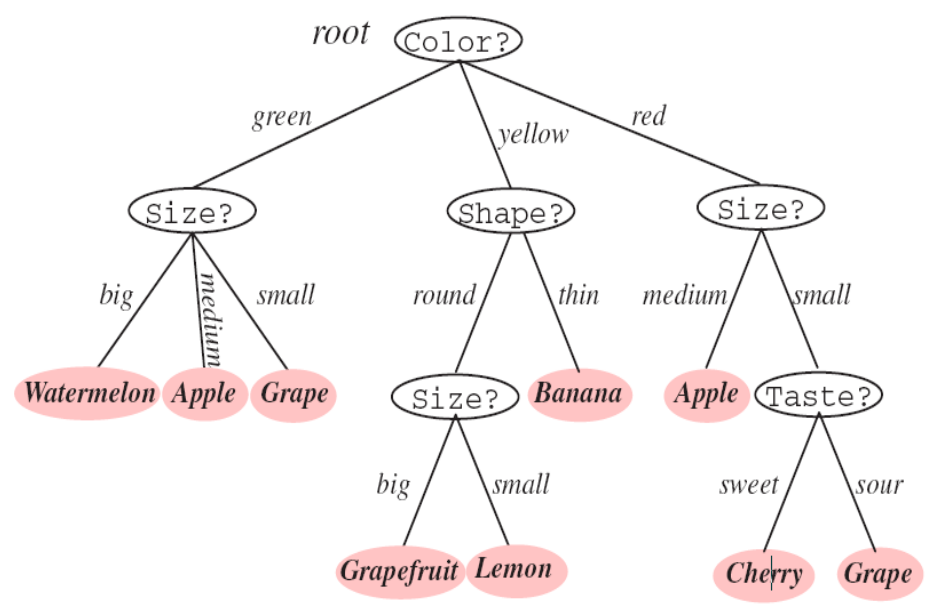
\includegraphics[scale=0.3,keepaspectratio]{tree}
\caption{Esempio di un albero decisionale}
\end{figure}
\subsection{Obiettivi}
Prima dell'inizio dello stage, Nextep ha redatto un \emph{Piano di Lavoro} contenente gli obiettivi da realizzare nelle settimane di \emph{stage}. Gli obiettivi erano suddivisi in minimi e massimi, successivamente in seguito ad una variazione delle priorità aziendali sono stati effettuati dei cambiamenti. Inizialmente, ho effettuato il \emph{porting} del modulo preesistente DRE, in modo che la persistenza fosse compatibile con OrientDb e che fosse compatibile con l'ultima versione di Play Framework. Visto il protrarsi delle attività di \emph{porting}, l'azienda ha deciso di sospendere il lavoro per poter lavorare sul nuovo modulo \emph{Tres}.
\newpage
Qui di seguito presento gli obiettivi dello stage:
\begin{itemize}
\item Obiettivi formativi
\begin{itemize}
\item Formazione sui sistemi di raccomandazione e degli algoritmi di apprendimento;
\item Studio delle tecnologie utilizzate, Scala e OrientDb;
\item Studio degli strumenti utilizzati, in particolar modo dei \emph{framework} e degli \emph{IDE}.
\end{itemize}
\item Obiettivi minimi
\begin{itemize}
\item Utilizzo del database OrientDb.
\end{itemize}
\item Obiettivi massimi
\begin{itemize}
\item Implementazione di nuovi modelli di algoritmi di apprendimento per migliorare l'individuazione dei gusti dell'utente;
\item Migliorare la fase di apprendimento del modello stesso;
\item Implementazioni di algoritmi di \emph{cluster} per il raggruppamento di elementi omogenei in un insieme di dati.
\end{itemize}
\end{itemize}
%**************************************************************************************************




%**************************************************************************************************
\section{Vincoli}
Questa sezione elenca i vincoli relativi al progetto di \emph{stage}.
\subsection{Vincoli temporali}
Per lo \emph{stage} i vincoli temporali sono imposti direttamente dall'università, essa stabilisce una durata minima di 300 ore e una durata massima di 320 ore. Per questo motivo ho modulato il \emph{Piano di Lavoro} in modo da distribuire le ore lavorative in 8 settimane. Con l'azienda ho concordato un impegno di 300 ore, divise in 37.5 ore settimanali. Le variazioni del piano sono state concordate con il \emph{tutor} aziendale in maniera da rispettare i vincoli temporali imposti in seguito a ritardi dovuti al \emph{porting} del modulo DRE.
\subsection{Vincoli metodologici}
Come strumento di versionamento ho scelto Git perché già utilizzato in precedenza e per il supporto che riceve da molti strumenti di sviluppo. Per la documentazione del codice ho scelto Scaladoc perchè viene fornito insieme al compilatore e similmente a Javadoc permette di documentare direttamente nel codice sorgente. Per il \emph{testing} nel progetto ho utilizzato TravisCI, esso fornisce un servizio di \emph{continuous integration} facilmente integrabile con i \emph{repository} di Github\footcite{https://github.com/}.
\begin{figure}[ht]
\centering
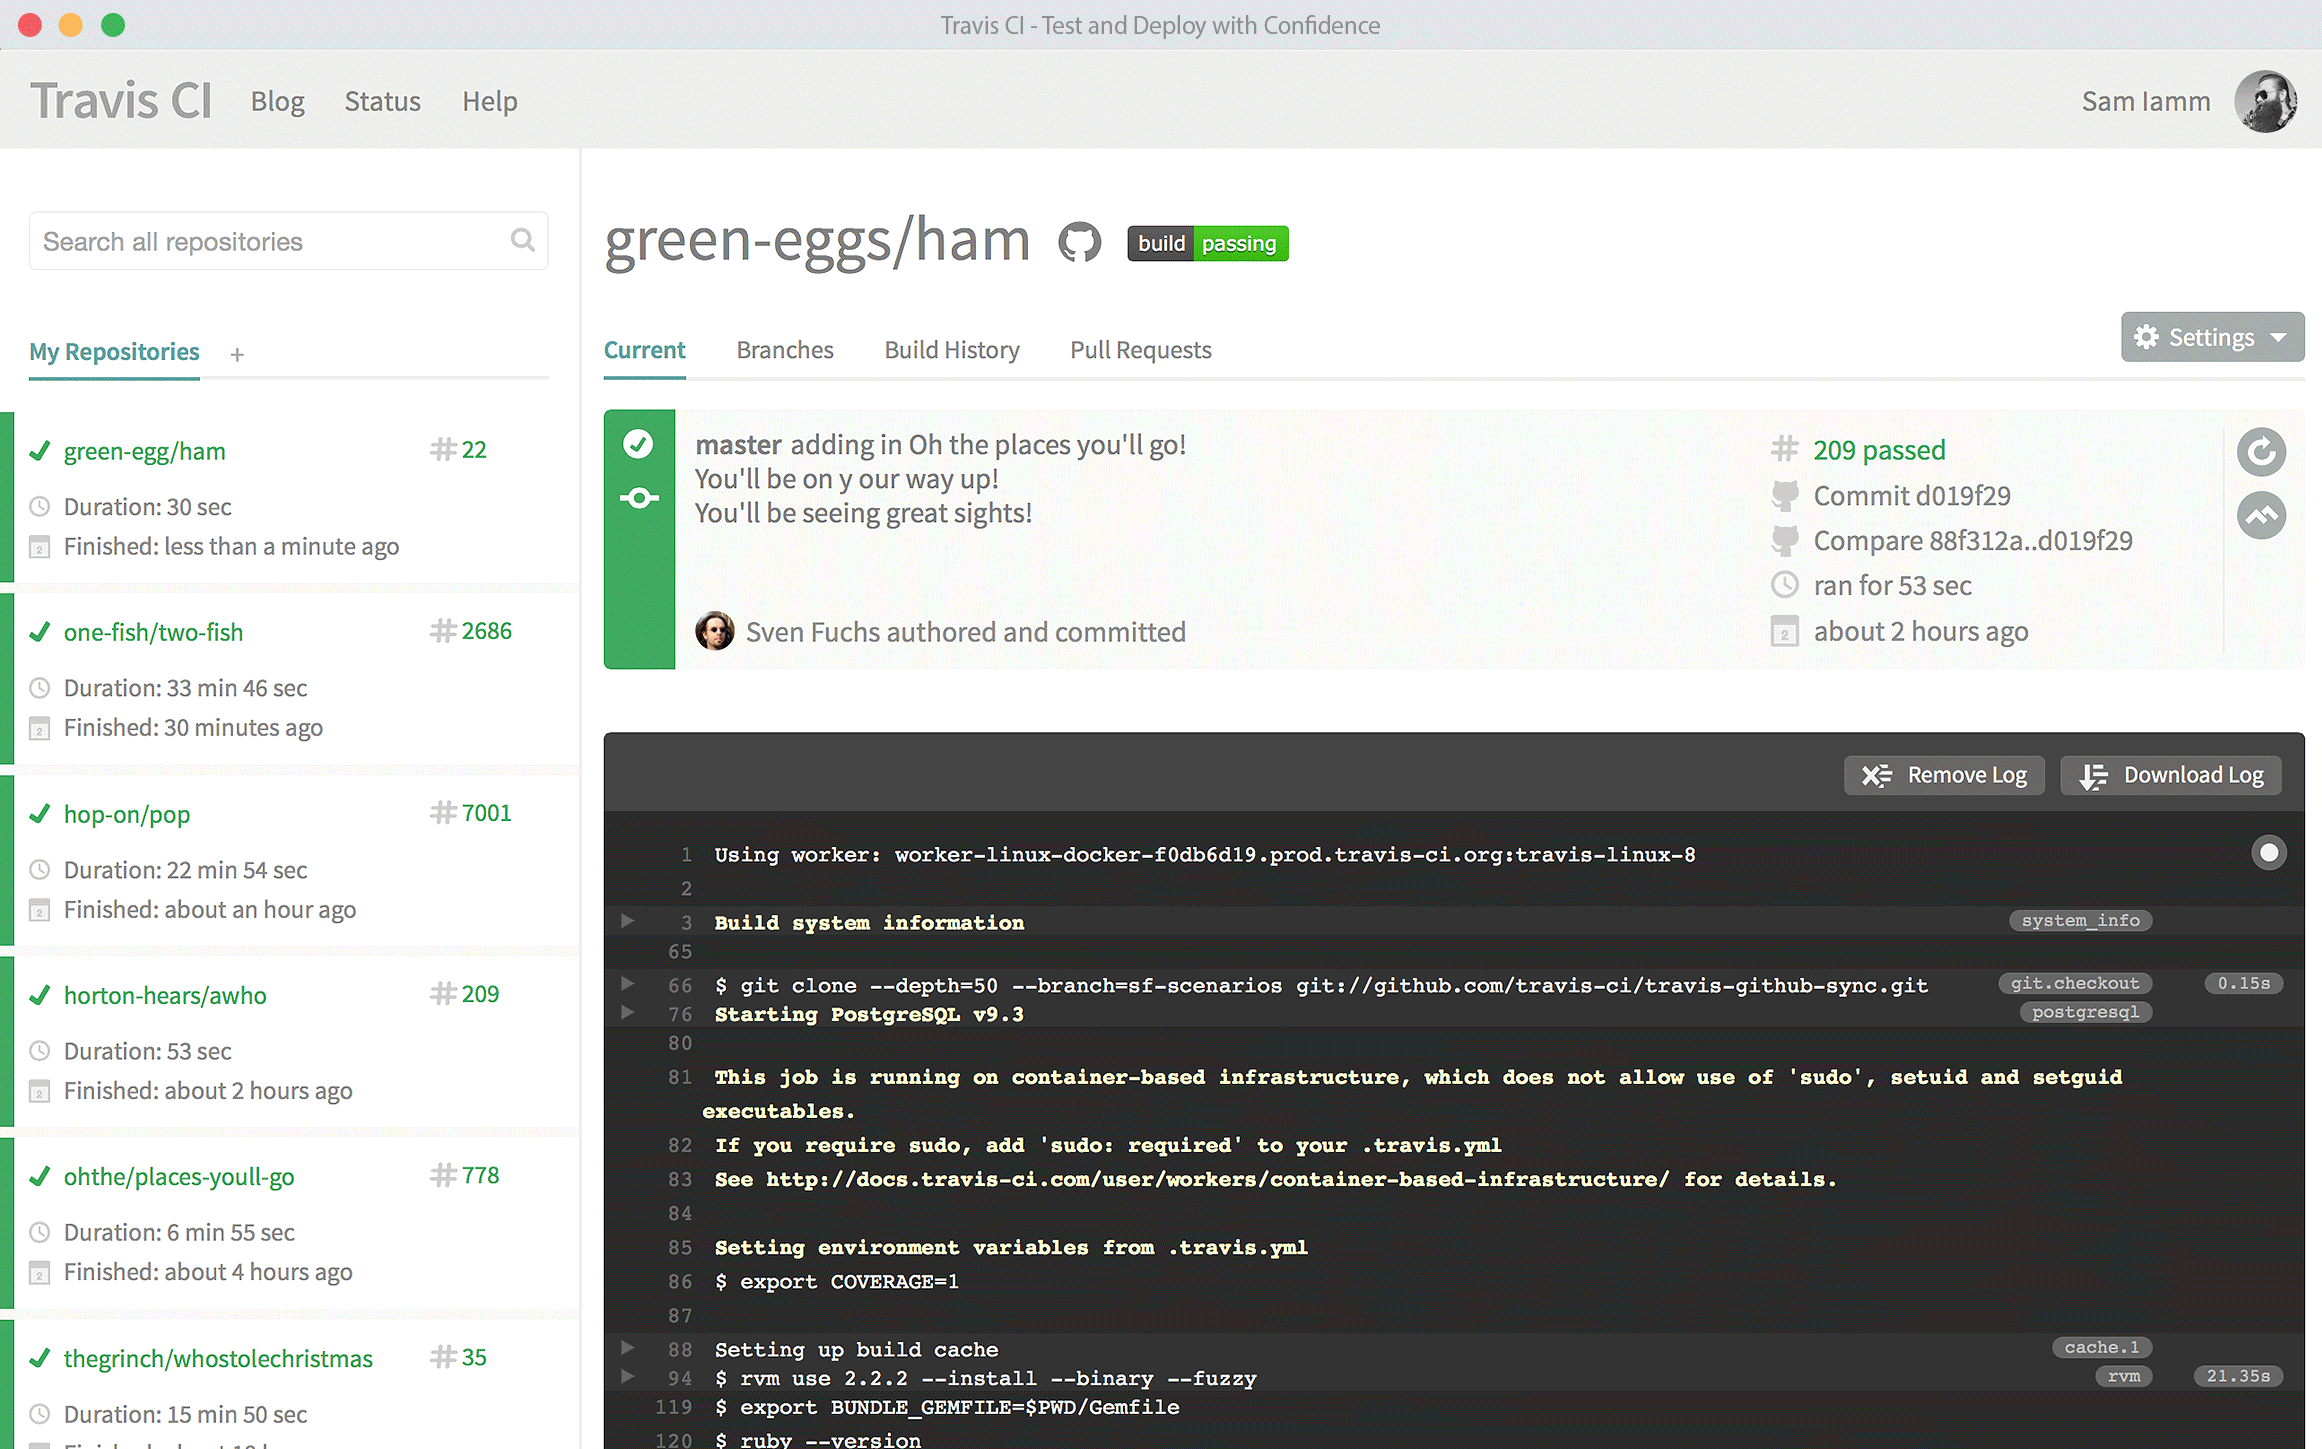
\includegraphics[scale=0.17,keepaspectratio]{travis}
\caption{Pannello di controllo travis}
\end{figure}
\newpage
Per lo sviluppo del codice ho scelto come \emph{IDE} IntelliJ in quanto:
\begin{itemize}
\item Già precedentemente utilizzato;
\item Ambiente di sviluppo compatibile con i maggiori linguaggi \emph{JVM-based};
\item Integrazione con Git;
\item Integrazione per lo sviluppo in Scala con Sbt.
\end{itemize}
Per la gestione progetti ho utilizzato il \emph{build tool} Sbt, perchè nell' ambiente di sviluppo di Scala è la scelta predominante ed è compatibile con il \emph{framework} utilizzato \emph{Play Framework}. Le caratteristiche distintive di questo \emph{framework} sono elencate di seguito:
\begin{itemize}
\item Definizione del file di configurazione in Scala;
\item Compatibilità con Scaladoc per documentazione;
\item Supporto per progetti misti Java/Scala;
\item Supporto per i maggiori \emph{tool} di \emph{testing};
\item Supporto per la gestione delle librerie.
\end{itemize}
Per la realizzazione dei diagrammi \emph{UML (Unified Modeling Language)} ho utilizzato Astah Professional\footcite{http://astah.net/}, uno strumento già utilizzato in precedenza e perché compatibile con gli ultimi standard \emph{UML 2.0}.
\subsection{Vincoli tecnologici}
\subsubsection{Scala}
Il principale linguaggio di programmazione adottato è Scala\footcite{http://www.scala-lang.org/} (acronimo di \emph{"Scalable Language"}). E' stato studiato per poter interoperare con \emph{Java Runtime Environment (JRE)}, quindi è possibile scrivere applicazioni sia in Java e Scala che eseguono nella stessa \emph{Java Virtual Machine (JVM)}. E' un linguaggio multi paradigma, che integra concetti provenienti dai linguaggi della programmazione ad oggetti e della programmazione funzionale. Scala è un linguaggio completamente \emph{object oriented}, infatti ogni elemento del linguaggio è un oggetto, compresi i tipi primitivi e le funzioni. Inoltre è un linguaggio funzionale, include funzioni di prima classe e una libreria con strutture dati immutabili efficienti.
\subsubsection{Play Framework}
Play è un \emph{framework} \emph{open source}, scritto in Java e Scala, che permette l'implementazione di \emph{web application} con il \emph{pattern model-view-controller}. Questo \emph{framework} trae ispirazione ed è simile a Ruby on Rails e Django.
\begin{figure}[ht]
\centering
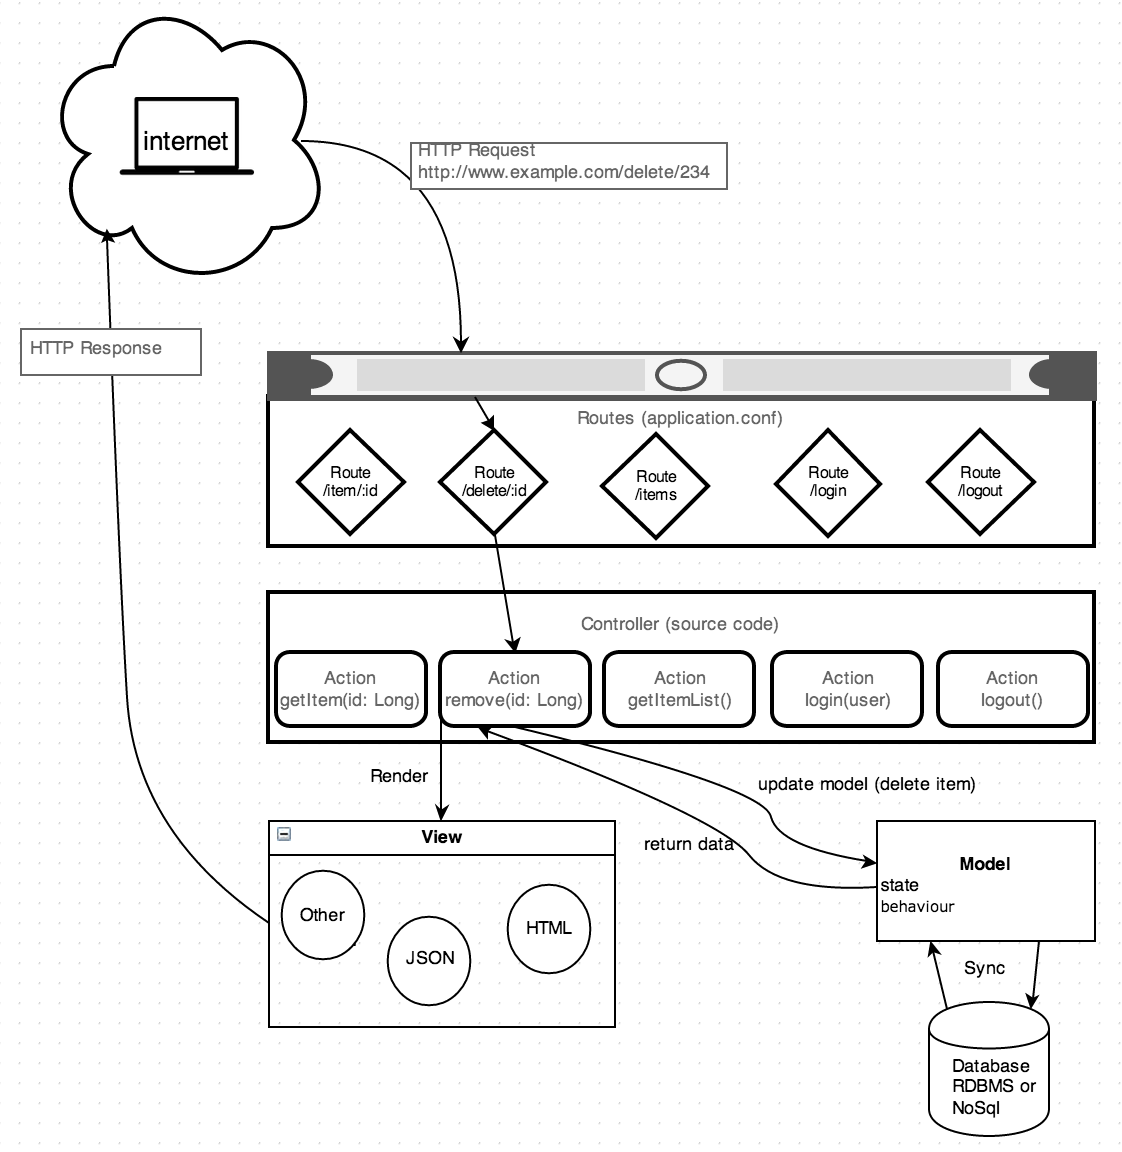
\includegraphics[scale=0.5]{immagini/play-arch}
\caption{Tipica architettura di un'applicazione che utilizza Play Framework. Immagine tratta da \href{https://110j.wordpress.com/2013/10/23/play-framework-2-1-architecture/}{Omer Haderi Blog}.}
\label{fig:play-app}
\end{figure}
\newpage
Le peculiarità che lo contraddistinguono dagli altri \emph{framework} sono le seguenti:
\begin{itemize}
\item Privo di stato: non viene mantenuta alcuna sessione sul server relativa ai dati dell'utente corrente;
\item Metodi statici: tutti i metodi dei \emph{controller} che vengono invocati dal \emph{framework} sono statici, o nel caso in cui si usi la versione Scala, sono funzioni di oggetti di Scala;
\item Gestione asincrona dell'\emph{input} e dell'\emph{output}: grazie all'uso di Netty Server, Play può gestire le richieste lunghe in modo asincrono;
\item Architettura modulare: come per Rails e Django, ci sono i moduli;
\item Supporto nativo per Scala: non solo Play è fatto internamente in Scala, ma espone anche delle interfacce Scala. Le interfacce Java sono state messe appositamente in \emph{package} diversi affinché possano seguire le convenzioni di Java.
\end{itemize}
Al suo interno permette una implementazione delle \emph{views}, specificando l'interfaccia con un linguaggio di \emph{markup} (e.g. Html, Xml, Json) in combinazione con del codice Scala. Vengono fornite molte classi di \emph{utility} come ad esempio Play Json Library che permette di operare con dei dati in formato Json, oppure un adattamento della libreria Specs2 che permette un supporto per il \emph{testing} di una applicazione in Play. Una tipica applicazione in Play funziona convogliando tutte le \emph{HTTP Request} nella componente \emph{Router} che invocherà a sua volta il \emph{Controller} pre-selezionato. Il \emph{Controller} interagisce con il \emph{Model} che a sua volta restituisce un risultato. In genere questo risultato verrà poi \emph{renderizzato} con la \emph{View} e fatto ritornare tramite un \emph{HTTP Response}.
\subsubsection{OrientDB}
Per la persistenza dei dati ho utilizzato OrientDb\footcite{http://orientdb.com/}, un \emph{Database Management System} (DBMS) multi-modello con una licenza \emph{open source}. Supporta i seguenti modelli di persistenza:
\begin{itemize}
\item \emph{Graph}: modello a grafo; 
\item \emph{Document}: modello a documenti come MongoDb;
\item \emph{Object}: modello ad oggetti che permette di memorizzare direttamente i \emph{POJO}.
\end{itemize}
Inoltre supporta modelli di definizione dello schema come \emph{schema-less}, \emph{schema-full} e \emph{schema-mixed}. Per motivi prestazionali non permette le \emph{join}, le relazioni sono gestite come in un database a grafo, ovvero delle connessioni dirette tra i \emph{record}. Questa caratteristica lo rende adatto nel contesto dei \emph{Big Data}, infatti la complessità computazionale per gestire una creazione di un \emph{link} è pari a O(1). Tra le caratteristiche più importanti di OrientDb:
\begin{itemize}
\item Scalabile: ovvero è possibile aggiungere al sistema un altro \emph{server} per aumentarne le prestazioni;
\item Transazionale: supporta transazioni completamente \emph{ACID} garantendo che tutte le transazioni  vengano processate in modo affidabile e nel caso di \emph{crash} viene ripristinato lo stato precedente(rollback);
\item Polyglot: supporta \emph{query} in un dialetto \emph{SQL-like}, oppure delle \emph{API REST} che forniscono l'accesso ai dati.
\end{itemize}
\begin{figure}[ht]
\centering
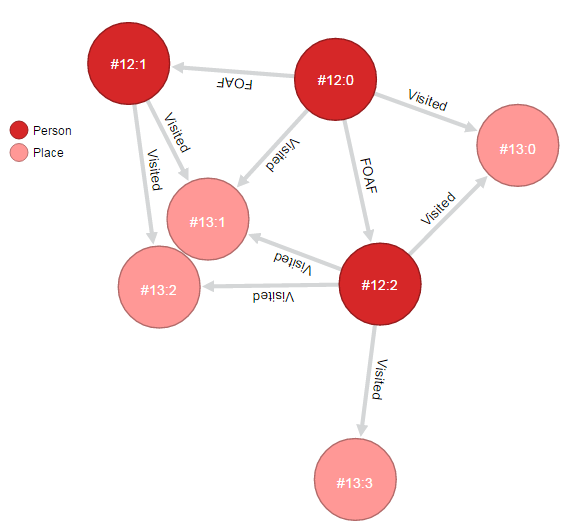
\includegraphics[scale=0.60]{immagini/graph_orientdb}
\caption{Esempio di modellazione in OrientDb. Immagine tratta da \href{http://blog.scalac.io/2015/11/26/orientdb-and-scala-part1.html}{Scalac Blog}}
\label{fig:orientdb-graph}
\end{figure}
%**************************************************************************************************




%**************************************************************************************************
\section{Obiettivi personali}
Questa sezione elenca gli obiettivi personali che hanno portato allo svolgimento dello \emph{stage}.\\Ho conosciuto l'azienda durante l'evento \emph{Stage-IT}. Questo evento mi ha dato la possibilità di approfondire molte proposte di \emph{stage}, da parte aziende provenienti da tutta la provincia di Padova e non. In seguito a tutte le proposte di \emph{stage} disponibili ho accettato la proposta di Nextep S.r.l. per i seguenti motivi:
\begin{itemize}
\item Il progetto permetteva di lavorare con tecnologie innovative che mi avrebbero fornito un valore professionale aggiunto;
\item Il progetto proposto era interessante perché toccava rami dell'intelligenza artificiale e dei sistemi di raccomandazione;
\item L'utilizzo di Scala, in modo da poter padroneggiare un linguaggio con un paradigma funzionale in forte ascesa di popolarità.
\end{itemize}
%**************************************************************************************************